\chapter{Solution Results}\label{solution}
This chapter illustrates the results of all implemented services and tools
created during this Master's Thesis by using a \ac{SysML} case study explained
in the preceding chapter. To achieve this all tools in the \ac{SEG}
pipeline are executed consecutively thus presenting the resulted integration of
\ac{UML} profiles using a real world example.

For testing the implemented solutions, one example scenario may be given
for this purpose.
Instead of using the \ac{PPU} scenarios 0 and 1 described in section~\ref{sysml:introduction}, the tools shall be tested with a more complex
revision change implemented in the \ac{SysML} case study.
Therefore both revision 2 and 3 are used, whereas the changes between them are
illustrated in figure~\ref{ppu_rev3}.

\begin{figure}[h!]
\begin{center}
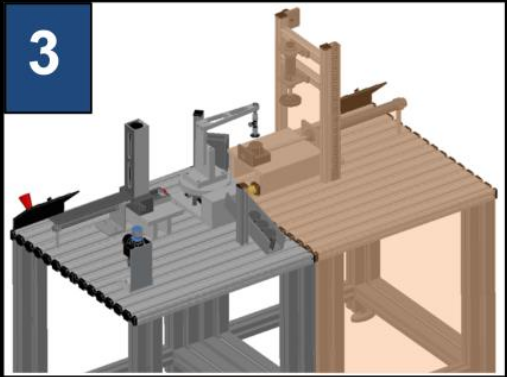
\includegraphics[scale=0.4]{ppu_rev3}\\
\end{center}
\caption{\ac{PPU} case study revision 3~\cite{aiscasestudy}}
\label{ppu_rev3}
\end{figure}

The important difference between both model revisions is the addition of a new
\textit{Stamp} module. Only metallic work pieces should be stamped, whereas
black plastic work pieces are transported to the slide without being processed. To implement such
semantics, there has to be an additional sensor for detecting the position of
the stamp, whereas revision 2 already contains the inductive sensor for
differentiating between the two kinds of work pieces. The stamping process
itself is straightforward as one can imagine the movement of the stamp module
consisting of up and down alterations. Finally the crane transports the stamped
or unprocessed work piece onto the slide. A view illustrating the relationship
described beforehand can be seen in figure~\ref{ppu_rev3_uml}.

\begin{figure}[h!]
\begin{center}
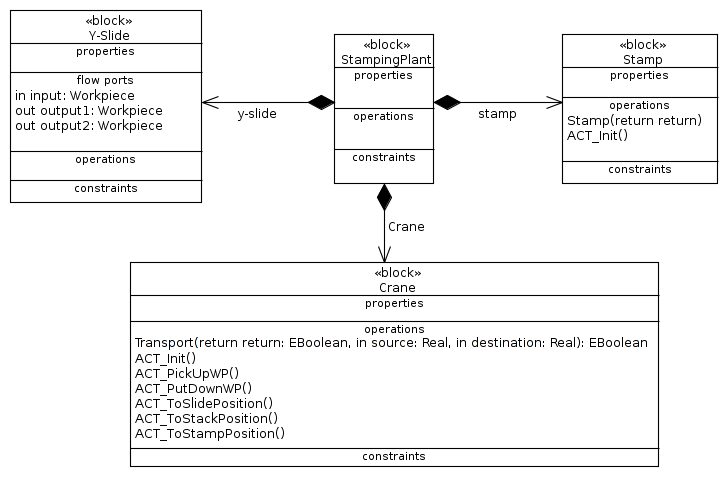
\includegraphics[scale=0.6]{ppu_rev3_uml}\\
\end{center}
\caption{Revision 3 \ac{UML} diagram snippet}
\label{ppu_rev3_uml}
\end{figure}

As described in the Diploma Thesis of Dennis Koch~\cite{kochThesis}, one
practical aspect of the creation and application of patches is the propagation
of changes throughout different versions of software like a product family.
Considering this use case one can imagine two different automation plants $P_1$ and
$P_2$ each consisting of mentioned \ac{PPU} at revision 2. In need of such
functionality the customer owning $P_1$ wants the provider of the
\ac{PPU} to integrate the described stamp module. As $P_1$ now equals to
revision 3 depicted in figure~\ref{ppu_rev3}, the owner of $P_2$ wants to
have the same functionality for his plant. Instead of developing the exact same
model the developer wants to reuse his work done in $P_1$. To achieve this goal
all developed tools in this Master's Thesis are used consecutively, divided into
steps explained in the following paragraphs. For a better overview the tool
pipeline is yet again depicted in figure~\ref{integration_overview2}, whereas
the used model instance $A_1$ corresponds to $P_1$ and $A_2$ to $P_2$
respectively.

\begin{figure}[h!]
\begin{center}
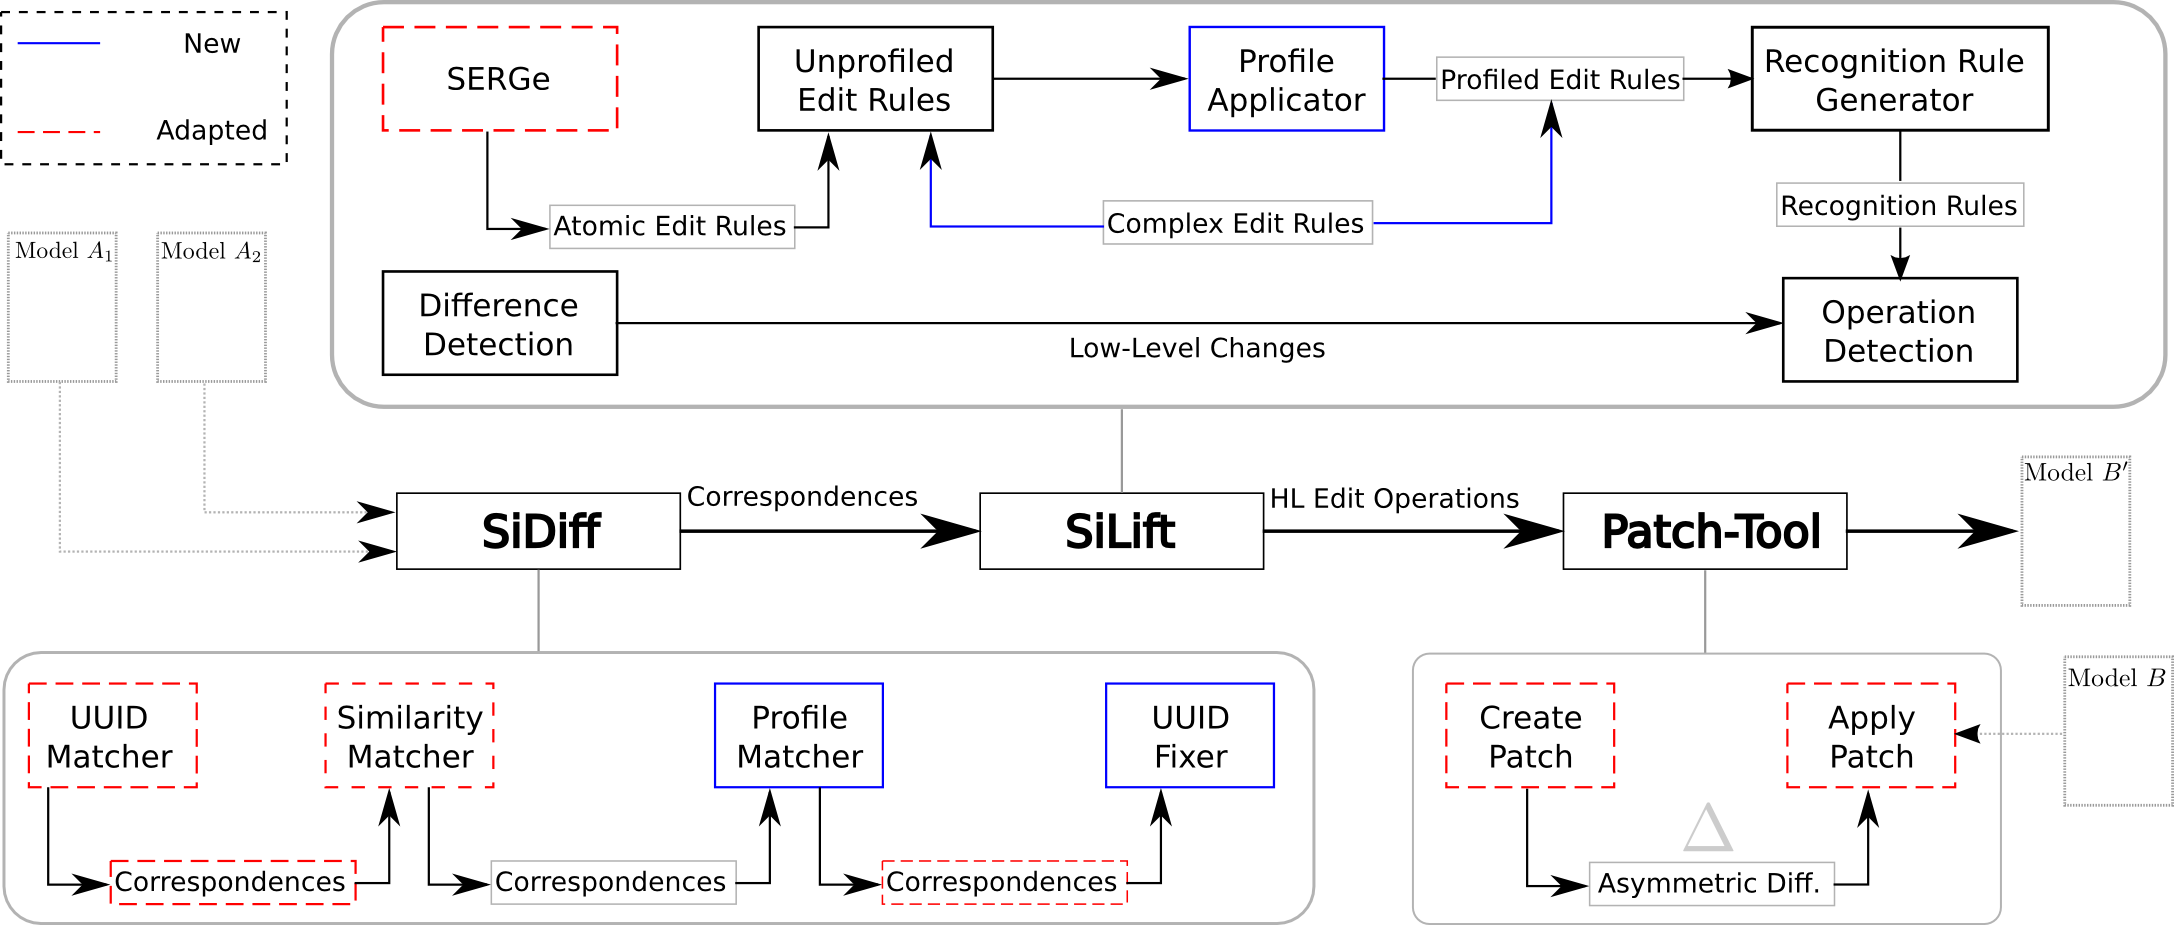
\includegraphics[scale=0.5, angle=0]{integration_overview}\\
\end{center}
\caption{UML profile integration overview}
\label{integration_overview2}
\end{figure}

\textbf{Compare $P_1$ and $P_2$} \\
The first step to the goal illustrated above is the detection of changes
between $P_1$ and the plant $P_2$. Using the SiDiff matching pipeline leads to
following results:
\begin{itemize}
  \item \textbf{\ac{UUID} Matcher}: 572 / 591 elements of $P_2$ matched, 785
  elements overall in $P_1$
  \item \textbf{Similarity Matcher}: 16 / 19 elements additionally matched
  \item \textbf{Profile Matcher}: 0 / 3 elements matched
  \item \textbf{Overall result}: 588 / 591 elements of $P_2$ matched, 197
  elements added in $P_1$
\end{itemize}

The first step matches all elements corresponding to their identifiers, whereas
in this example almost all elements could be matched already in this first
matching step. Using the \ac{UUID} matcher at first in this particular
case therefore leads to better results in the following similarity matching
phase. In this second matcher additionally 16 elements are matched according to their similarity. The final matching step for
profiled elements does not add any matches, as the remaining 3 elements are
originated from pure \ac{UML}. In the overall result for almost all elements of
$P_2$ have correspondences been found in $P_1$ which translates to only 3 delete
operations compared to $P_2$. Additionally 197 elements have been found in $P_2$
which correlates to newly added model elements in comparison to $P_1$. 
\newpage
\textbf{Analyze computed difference} \\
As the addition of a stamp block includes many other changes as well, the
developer now wants to analyze the detected differences and changes in detail.
First SiLift will derive low-level changes from the symmetric difference
computed by SiDiff. There are 764 low-level changes detected between $P_1$
and $P_2$ which need to be analyzed now if not lifted afterwards. To cope with
this many computed low-level changes the SiLift tool will lift this difference 
into a more meaningful list of edit operations. As seen in the center of
figure~\ref{integration_overview2}, SiLift now makes use of the profiled edit
rules created through the \textit{ProfileApplicator} as well as the manually
created edit rules. Using a complete rule base created earlier
for lifting will recognize edit operations like the manually created
depicted in figure~\ref{create_association_operation} and the profiled one in
figure~\ref{create_block_operation}.

\begin{figure}[h!]
\begin{center}
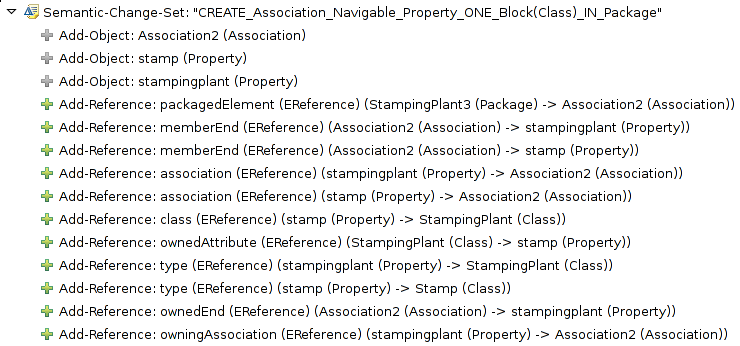
\includegraphics[scale=0.5]{create_association_operation}\\
\end{center}
\caption{Recognized manually created edit operation}
\label{create_association_operation}
\end{figure}

Low-level changes which are contained in such \ac{SCS}s will ease the
understanding of made changes as clearly presented in
figure~\ref{create_association_operation}: 14 low-level changes have been
grouped together into 1 meaningful edit operation, the creation of an
association which is navigable in one end that is.

\begin{figure}[h!]
\begin{center}
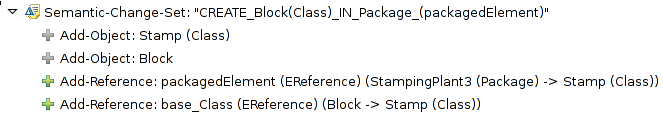
\includegraphics[scale=0.5]{create_block_operation}\\
\end{center}
\caption{Recognized profiled create operation}
\label{create_block_operation}
\end{figure}
\newpage
A result summary of all lifted low-level changes detected is
presented in the following table which reduces the number to 231 edit
operations instead of 758 low-level changes.\\
\begin{center}
{\footnotesize
\begin{tabular}{|l|r|}
Edit Operation & Amount\\
\hline
CREATE\_Transition\_IN\_Region\_(transition) & 49\\
CREATE\_State\_IN\_Region\_(subvertex) & 27\\
SET\_Transition\_(guard)\_TGT\_Constraint & 24\\
ADD\_Operation\_(method)\_TGT\_Behavior & 19\\
CREATE\_Constraint\_IN\_Transition\_(ownedRule)\_LiteralString\_ & 19\\
CREATE\_Activity\_IN\_State\_(doActivity) & 14\\
CREATE\_OpaqueBehavior\_IN\_State\_(doActivity) & 8\\
CREATE\_Pseudostate\_IN\_Region\_(subvertex) & 7\\
CREATE\_FinalState\_IN\_Region\_(subvertex) & 6\\
CREATE\_OpaqueBehavior\_IN\_State\_(entry) & 6\\
CREATE\_OpaqueBehavior\_IN\_Transition\_(effect) & 5\\
CREATE\_Association\_Navigable\_Property\_ONE\_Block(Class)\_IN\_Package & 5\\
UNSET\_Transition\_(guard)\_TGT\_Constraint & 4\\
CREATE\_Constraint\_IN\_Transition\_(ownedRule)\_LiteralBoolean\_ & 4\\
CREATE\_OpaqueBehavior\_IN\_State\_(exit) & 3\\
CREATE\_Operation\_IN\_Block(Class)\_(ownedOperation) & 3\\
SET\_Association\_Name & 3\\
SET\_State\_Name & 3\\
CREATE\_StateMachine\_IN\_Block(Class)\_(ownedBehavior) & 3\\
SET\_OpaqueBehavior\_Name & 2\\
SET\_Region\_Name & 2\\
DELETE\_Transition\_IN\_Region\_(transition) & 1\\
REMOVE\_Operation\_(method)\_TGT\_Behavior & 1\\
SET\_LiteralString\_Name & 1\\
DELETE\_Constraint\_IN\_Transition\_(ownedRule)\_LiteralString\_ & 1\\
MOVE\_Constraint\_(ownedRule)\_Transition & 1\\
SET\_Constraint\_Name & 1\\
CREATE\_Region\_IN\_State\_(region) & 1\\
MOVE\_State\_FROM\_Region\_(subvertex)\_TO\_Region\_(subvertex) & 1\\
SET\_Package\_Name & 1\\
CREATE\_Parameter\_IN\_Operation\_(ownedParameter) & 1\\
SET\_LiteralString\_Value & 1\\
SET\_Activity\_Name & 1\\
DELETE\_OpaqueBehavior\_IN\_State\_(doActivity) & 1\\
CREATE\_Block(Class)\_IN\_Package\_(packagedElement) & 1\\
\hline
 & \textbf{231} \\
\end{tabular}
}
\captionof{table}{SiLift lifting result summary}
\end{center}

\textbf{Create a patch} \\
Using the Patch-Tool the developer now wants to create a patch containing all
edit operations presented in the previous table. As the rule base is complete and all
low-level changes have been lifted by SiLift previously, all dependencies
between these are considered additionally. One example of such dependency
detected is illustrated in figure~\ref{dependency_example}: To create a
transition connecting two states both states have to be created first.

\begin{figure}[h!]
\begin{center}
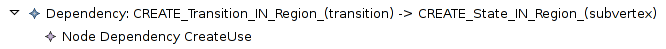
\includegraphics[scale=0.5]{dependency_example}\\
\end{center}
\caption{Detected create-use dependency example}
\label{dependency_example}
\end{figure}

\textbf{Apply the created patch} \\
The next step is to apply the patch created beforehand to plant $P_2$, as this
plant shall implement the changes of $P_1$ compared to $P_2$. The application is
straightforward as presented in~\cite{kochThesis} and shall not be explained in
detail.

\textbf{Validate the resulted model} \\
The final step is to validate the resulted model. The developer wants to assure
that
\begin{itemize}
  \item[a)] the patch has applied all changes consistency preserving and that
  \item[b)] the resulted model equals to the expected result.
\end{itemize}

As the patch creation already assures a), the final step is to test the model
for its semantically correctness. To check for equality between $P_1$ and $P_2$
described in b) the SiDiff matching pipeline is used again and must report no
differences and all elements shall correspond as already presented in
figure~\ref{patch_correctness}.

\textbf{Final result} \\
The patch containing all changes could successfully be created and applied and
resulted in an equal plant implementing the stamp module, which is the desired
result. The patch can now be applied to different \ac{PPU}s for integrating such
new module.

Additionally to this example scenario between revision 2 and 3 of the \ac{PPU}
in the course of this Master's Thesis a batch application for testing all steps
above has been adapted for \ac{SysML}. The idea is to execute all steps for
consecutive revisions and log all results, which are shown in the
following table and correspond to the graphs in
figure~\ref{revisionChanges_analysis}.

\begin{center}
{\footnotesize
\begin{tabular}{|c|c|c|c|c|}
Revision Change & Correspondences & Differences & Operations & Equal\\
\hline
00$\rightarrow$01 & 545 & 58 & 16  & {\color{green}Yes} \\
01$\rightarrow$02 & 545 & 203 & 86  & {\color{green}Yes} \\
02$\rightarrow$03 & 575 & 764 & 231  & {\color{green}Yes} \\
03$\rightarrow$04 & 774 & 9 & 9  & {\color{green}Yes} \\
04$\rightarrow$05 & 756 & 654 & 201  & {\color{green}Yes} \\
05$\rightarrow$07 & 904 & 165 & 102  & {\color{green}Yes} \\
07$\rightarrow$08 & 927 & 103 & 28  & {\color{green}Yes} \\
08$\rightarrow$09 & 943 & 298 & 94  & {\color{green}Yes} \\
09$\rightarrow$10 & 1008 & 367 & 111  & {\color{green}Yes} \\
10$\rightarrow$11 & 1099 & 83 & 28  & {\color{green}Yes} \\
11$\rightarrow$12 & 1107 & 436 & 143  & {\color{green}Yes} \\
12$\rightarrow$13 & 1216 & 95 & 40  & {\color{green}Yes} \\
\hline
\end{tabular}
}
\captionof{table}{Batch-Patch summary report}
\end{center}

As illustrated in the table all revision changes can be handled now in all
tools in the \ac{SEG} pipeline, whereas all resulting patched models are equal
to their corresponding revision. The final conclusion of these results is
presented in the following chapter.